\documentclass[reprint,nofootinbib,...]{revtex4-1} 
%\documentclass[draft,nofootinbib,...]{revtex4-1} 
\usepackage{amsmath}%
\usepackage{amsthm,amssymb}
\usepackage{graphicx}
\usepackage{epstopdf}
\usepackage{xcolor}
\usepackage{algcompatible}
\usepackage[size=small]{caption}
\usepackage{etoolbox}
\usepackage{booktabs}
\usepackage{multirow}
\usepackage[utf8]{inputenc}
\usepackage[colorinlistoftodos]{todonotes}

\usepackage[hyperfootnotes=true]{hyperref}
\hypersetup{
 colorlinks=true,
 citecolor=blue,
 linkcolor=blue,
 urlcolor=blue}

%%% ----------------------------------------------------------------------
\begin{document}

%Title of paper
\title{AI Safety for High Energy Physics}

\author{Benjamin Nachman}
\email{bpnachman@lbl.gov}

\affiliation{Physics Division, Lawrence Berkeley National Laboratory, Berkeley, CA 94720, USA}

\author{Chase Shimmin}
\email{chase.shimmin@yale.edu}

\affiliation{Department of Physics, Yale University, New Haven, CT 06511, USA}

\begin{abstract}
Since the first application of deep learning on `low-level' features for classification in high energy physics (HEP)~\cite{Baldi:2014kfa}, there has been a rapidly expanding literature on the adaptation of industrial deep learning techniques as well as the development of novel methods.  The overall conclusion from this impressive and extensive set of studies is that rarer and more complex signatures can be identified with the new set of powerful tools from deep learning.  However, there is an unstudied risk associated with the traditional HEP workflow and deep learning with high-dimensional data.  In particular, calibrating and validating deep networks in their natural high dimensionality is not possible and therefore current methods may be biased in ways that are not covered by current uncertainty estimates.  By borrowing ideas from AI safety, we illustrate these potential issues and propose a method to blah.  Last sentence.
\end{abstract}

\date{\today}
\maketitle

%%%%%%%%%%%%%%%%%%%%%%%%%%%%%

In collider-based high-energy physics (HEP), simulations modeling length scales from sub-nuclear reactions all the way to macroscopic scales are critical for scientific inference by connecting fundamental theories to observable quantities.  These simulations are excellent, but are an approximation to nature and therefore must be calibrated with data. In the quest for new particles, calibrated simulations of the Standard Model (SM) are compared with data to search for potential deviations.

In the traditional paradigm, a discriminating observable $m$ is used to isolate a region of phase space $m<c$ where contributions from new particles are expected to be small compared with the SM background processes.  In this \textit{control region}, the predicted cross-section is scaled to match the data and then the scaled differential cross-section from simulation is used to estimate the Standard Model contribution in a \text{signal region} with $m\gg c$.  Theoretical uncertainties on the extrapolation are estimated by repeating this procedure with a variety of simulations.

Deep learning offers a new set of tools in HEP for seeking out new particles using high-dimensional, low-level information~\cite{Baldi:2014kfa,Larkoski:2017jix,Radovic:2018dip,Guest:2018yhq}. A growing number of searches at the Large Hadron Collider are using deep learning methods to construct $m$. The control region method is the baseline approach for estimating the SM background in the nascent deep learning era.

A potential problem of the control region method with deep learning is that the calibration procedure may not sufficiently probe the high dimensionality of the feature space.  For example, if $\mathcal{O}(1000)$ dimensions are used for training a neural network, but only $\mathcal{O}(1)$ simulation variations are considered for the uncertainty on the calibration (as is common), then the prediction in the signal region may be incorrect: the uncertainty may be much smaller than the potential bias.

In this work, we use methods from AI safety to diagnose the sensitivity of the current methodology to 

To illustrate, introduce example and simulation, ...

As a first step, FGSM~\cite{DBLP:journals/corr/GoodfellowSS14}, ...

\begin{figure}[h!]
\centering
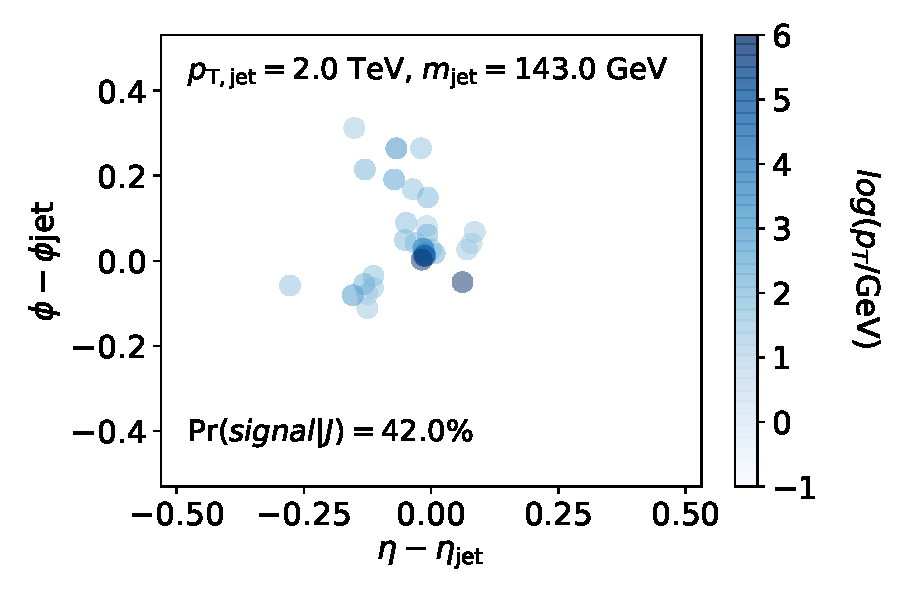
\includegraphics[width=0.23\textwidth]{figures/panel_1.pdf}
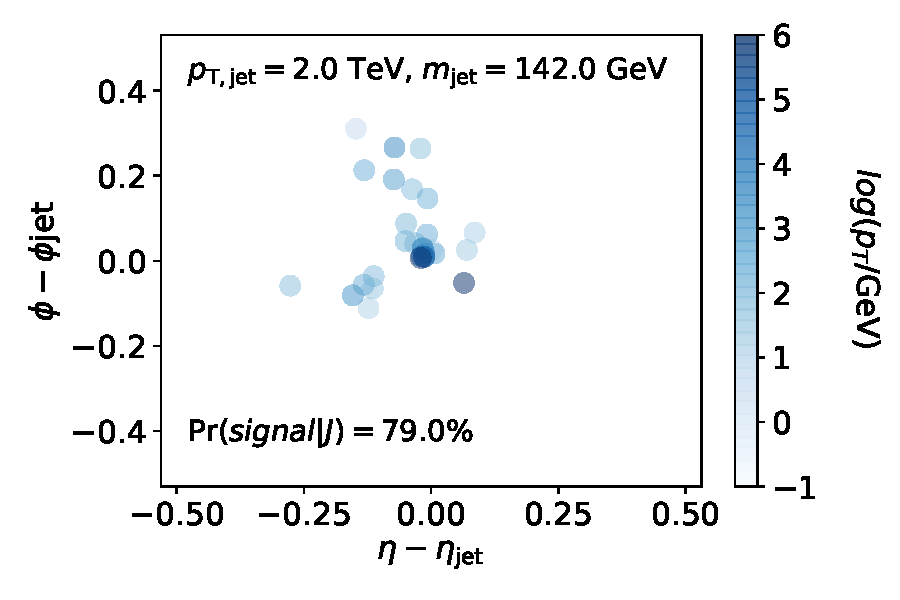
\includegraphics[width=0.23\textwidth]{figures/panel_2.pdf}
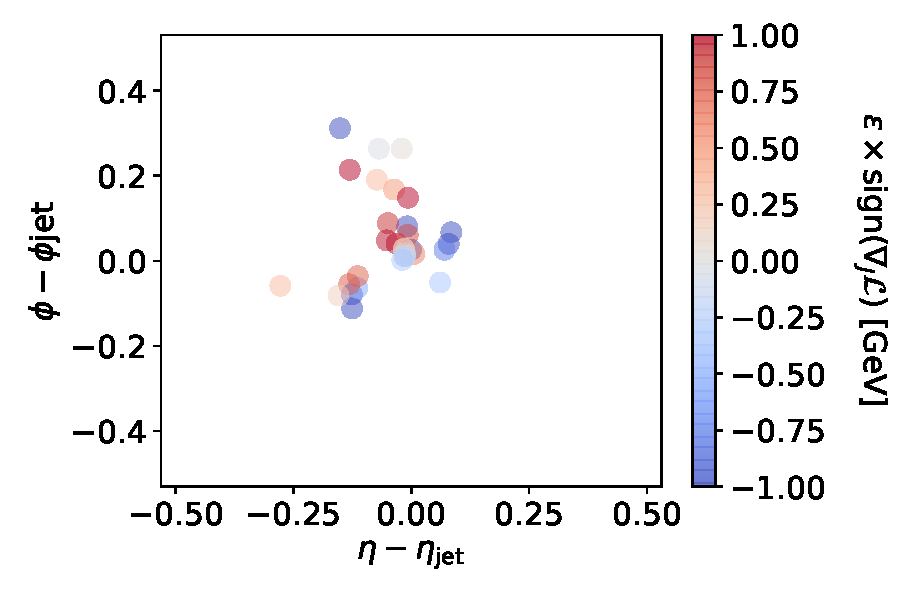
\includegraphics[width=0.23\textwidth]{figures/panel_3.pdf}
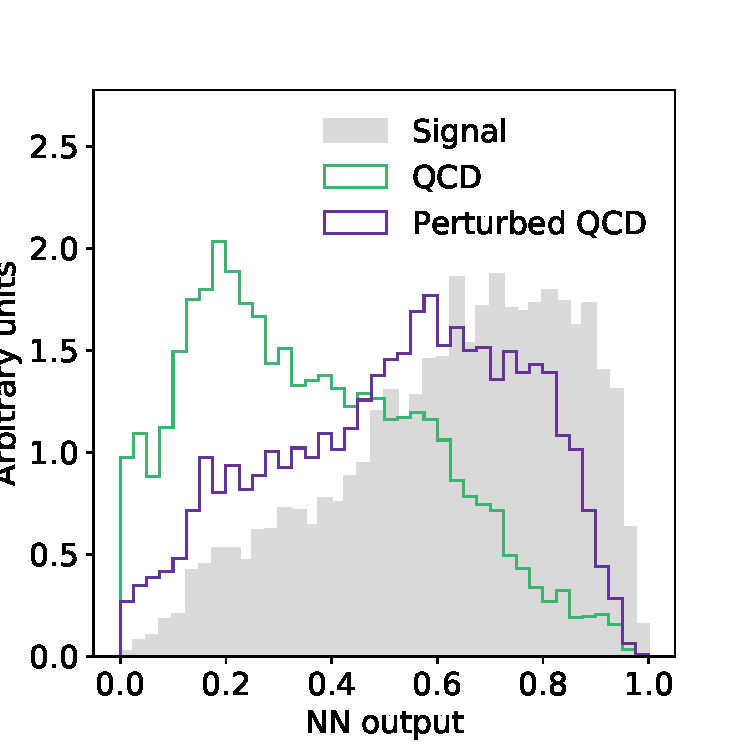
\includegraphics[width=0.2\textwidth]{figures/NN_FGSM.pdf}
\label{fig:FGSM}
\caption{Individual jet adversary.}
\end{figure}

(Talk about IRC safe inputs with FGSM, ...)

While the FGSM illustrated that single events can be attacked, ...

Talk about IRC safe inputs, ...

Conclusion...


\section*{ACKNOWLEDGMENTS}

This work is supported by the DOE under contract DE-AC02-05CH11231. 

\bibliography{myrefs}

\end{document}